\section{Durchführung}
\label{sec:Durchführung}
Für die einzelnen Teile des Versuches werden
Spule und Kondensator unverändert gelassen, der Widerstand wird im Verlauf
der Messungen variiert.
Zunächst werden Eigenschaften des gedämpften Schwingkreises bestimmt,
im speziellen der effektive
Dämpfungswiderstand aus dem zeitlichen Amplitudenverlauf
sowie der Dämpfungswiderstand, bei dem die aperiodische
Dämpfung auftritt.

Im ersten Fall sei der Widerstand konstant und der Schwingkreis wird durch eine
Rechteckspannung angeregt. Durch geeignete Wahl der Frequenz lässt sich ein
gedämpfter Schwingkreis ohne Anregung simulieren. Der Spannungsverlauf wird
an einem Oszilloskop aufgezeichnet und zur Auswertung abgespeichert.
\begin{figure}
  \centering
  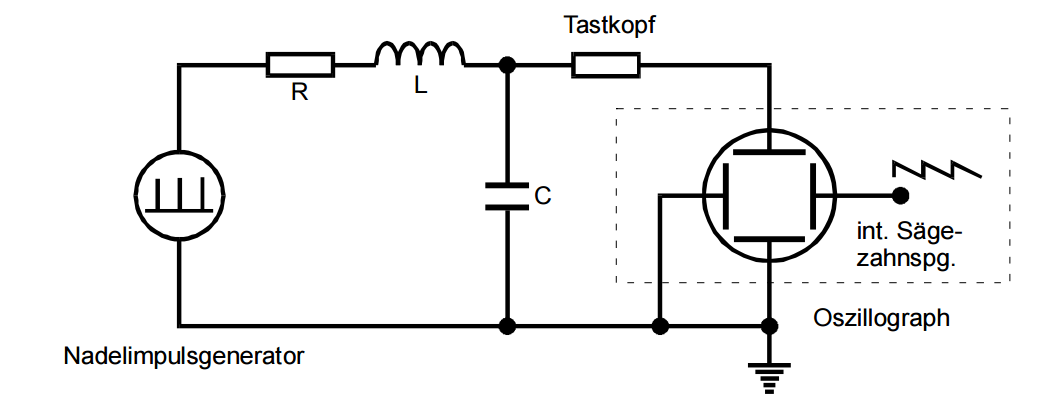
\includegraphics[keepaspectratio, width=\textwidth]{5a.png}
  \caption{Schaltung zur Untersuchung der Zeitabhängigkeit
  der Amplitude \cite{officialmanual}.}
  \label{fig:5a}
\end{figure}
Die verwendete Schaltung ist in Abbildung \ref{fig:5a} dargestellt. Anstelle des
Nadelimpulsgenerators wird die erwähnte Rechtecksspannung verwendet.

Für den zweiten Versuchsteil wird der feste Widerstand $R$ durch einen auf bis zu
\SI{10}{\kilo\ohm} regelbaren ersetzt. Dieser Widerstand wird zunächst auf seinen
Maximalwert eingestellt und dann verringert, bis der Spannungsverlauf
auf dem Oszilloskop dem des aperiodischen Grenzfalles entspricht
(siehe Abb.\ref{fig:aper}).

Für die weiteren Versuchsteile wird der regelbare Widerstand wieder durch einen
festen Widerstand ersetzt und die anregende Spannung zu einer sinusförmigen
Wechselspannung geändert. Die Amplitude bleibt über alle Messungen konstant,
die Frequenz wird geändert um die Frequenzabhängigkeit von Amplitude und
Phasenverschiebung nachzuweisen.
Gemessen werden bei verschiedenen Frequenzen die Erreger- und
Kondensatorspannung sowie die Phase zwischen beiden.

Dafür werden die Amplitude von Kondensator- und Erregerspannung für jede
Frequenz einzeln mit dem Tastkopf gemessen,
weil die Messung durch den Frequenzgang der Tastkopfes beeinflusst werden kann.
Um die Phase zu messen werden beide Spannungen gegeneinander am Oszilloskop
aufgetragen und die Zeitdifferenz zwischen zwei Extrema
oder ähnlich ausgezeichneten Punkten bestimmt.
